%%%%%%%%%%%%%%%%%%%%%%%%%%%%%%%%%%%%%%%%%%%%%%%%%%%%%%%%%%%%%%%%%%%%%%%%%%%%%%%%

% IEEEconf.cls file must exist in the same directory as the TeX file you want to compile
\documentclass[letterpaper, 10 pt, conference]{IEEEconf}

\title{\LARGE \bf
COMPUTER HISTORY\\
\large Group Topic Expressed In A Few Words
}

\author{Group Number\\
\small Group Member 1\\
\small Group Member 2\\
\small Group Member 3\\
}

% Image/graphics support
\usepackage{graphicx}
\graphicspath{ {./images/} }

% Formatting for lists
\usepackage{enumitem}

% Formatting for media
\usepackage{float}
\restylefloat{table}
\restylefloat{figure}

\begin{document}


\maketitle
\thispagestyle{empty}
\pagestyle{empty}


%%%%%%%%%%%%%%%%%%%%%%%%%%%%%%%%%%%%%%%%%%%%%%%%%%%%%%%%%%%%%%%%%%%%%%%%%%%%%%%%
\section*{ABSTRACT}
\textit{
This document is a basic template for writing conference-style
reports in LaTeX. You will use this template when writing
your report; you will need to replace all text (excluding
section headers or preamble information) with the content
of your report.
}

%%%%%%%%%%%%%%%%%%%%%%%%%%%%%%%%%%%%%%%%%%%%%%%%%%%%%%%%%%%%%%%%%%%%%%%%%%%%%%%%
\section{INTRODUCTION}

This document is an example of Assignment 3 in CSE/IT101.
You should describe what topic you chose and
why you chose that topic. Also provide a summary of the
topic, in a general sense. This section should describe any
background information that the reader needs to know to
understand your topic.

%%%%%%%%%%%%%%%%%%%%%%%%%%%%%%%%%%%%%%%%%%%%%%%%%%%%%%%%%%%%%%%%%%%%%%%%%%%%%%%%
\section{TIME PERIOD}

You should describe the time period in which your topic was
invented or used here. Also include the context for why your
topic was created or for how it is used. Any specific historical
information should be included here.

%%%%%%%%%%%%%%%%%%%%%%%%%%%%%%%%%%%%%%%%%%%%%%%%%%%%%%%%%%%%%%%%%%%%%%%%%%%%%%%%
\section{COMPUTER HARDWARE}

You should list the specification of any hardware your topic
uses here. If you want make a table here, please label the table
and include discussion on what components are included in the
table and why. See Table
\ref{tbl:example} for an example of a table.
The labels/captions of the table should be put at the bottom
of the table.


\begin{table}[h!]
\begin{center}
\begin{tabular}{||c | c | c | c||} 
\hline
  & Col1 & Col2 & Col3 \\ [0.5ex]
\hline\hline
Row1 & (1,1) & (1,2) & (1,3) \\ 
\hline
Row2 & (2,1) & (2,2) & (2,3) \\
\hline
Row3 & (3,1) & (3,2) & (3,3) \\
\hline
\end{tabular}
\caption{Example of a table}
\label{tbl:example}
\end{center}
\end{table}

You might want to put figures in the document. Please
remember to label them. The labels/captions of the figures
should be put at the bottom of the figure. See Figure
\ref{fig:example} for an example of how to use figures.
You will need to place the figure in an \texttt{images/} folder
in your working directory.

\begin{figure}[h!]
\centering
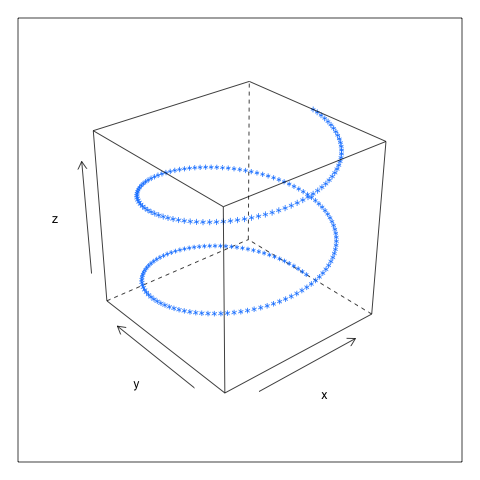
\includegraphics[width=0.5\textwidth]{spiral.png}
\caption{Example of a figure}
\label{fig:example}
\end{figure} 

\section{COMPUTER SOFTWARE}

Describe the software used for your chosen topic if any,
and state any uses of the software that your topic had.
If your topic does not have or use software, describe why it
doesn't use software and how it functions without it.

\section{CONCLUSION}

Conclude your research paper with any reflections on what you
learned about your topic. Was this what you expected to find?
Did you find any facts that surprised you? You may add other
personal reflections about the topic here.

\section*{REFERENCES}

Below are basic formats for different types of references.

\begin{enumerate}[label={[\arabic*]}]
\item Name of Author, ``Title of chapter in the book,''
Title of The Published Book, xth edition. City of
Publisher, Country if not U.S.
\item Name of Author, “Name of paper,” Abbrev.
Title of Periodical, vol. x, no. x, pp. xxx-xxx,
Abbrev. Month, year.
\item Name of Author, (Year, Month),
Title of Internet Article [Online]. Available E-Mail:
E-Mail.
\end{enumerate}

\end{document}

